\documentclass{report}
\usepackage[utf8]{inputenc}
\usepackage{pdfpages}
\usepackage{hyperref}
\usepackage{graphicx}
\usepackage{float}


\title{Datalogger Documentation}
\graphicspath{{./Images/}}
\author{Huy Trinh }
\date{August 2021}

\begin{document}

\begin{titlepage}
\maketitle
\end{titlepage}



\section{Overview}

The datalogger configuration includes\\
\\\textbf{Raspberry Pi 3 Model B + Vectornav VN200}
\\
\\These can be found through these links
\begin{enumerate}
    \item RPi: \url{https://www.raspberrypi.org/products/raspberry-pi-3-model-b/}
    \item VectorNav
    \begin{enumerate}
        \item[2.1] Quick start manual:\url{https://www.vectornav.com/docs/default-source/datasheets/vn-200-datasheet-rev2.pdf?sfvrsn=e1a7b2a0_10}
        \item[2.2] Complete manual page: \url{https://2w6vmg3m8cv83pn80b2dfi9f-wpengine.netdna-ssl.com/wp-content/uploads/assets/1/7/VN200UserManual_UM004_080514.pdf}
    \end{enumerate}
    \item PoEHat: \url{https://www.raspberrypi.org/products/poe-hat/}
\end{enumerate}
The GNSS/VectorNav connects to the mainboard (Raspberry Pi) through UART serial connection.

\section{Hardware}
\subsection{Circuit}
The USB power input is connected to 5V pins along with GNSS power. GNSS data is connected to UART pins. Power switch is connected between GPIO18 (BCM) and ground, pullup enabled in software. Primary LED (blue) is connected to GPIO24 (BCM), secondary LED (green) is connected to GPIO25 (BCM) and tertiary LED (red) is connected to GPIO10 (BCM). All the LEDs are driven with MOSFETs/NPN-transistors.More detail can found at: \url{https://tinyurl.com/ygbxmabs} 
\begin{figure}[H]
    \centering
    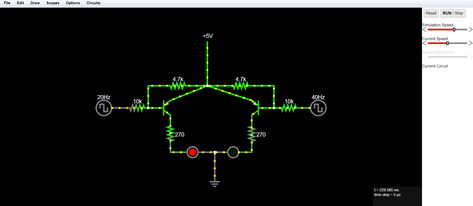
\includegraphics[width=\textwidth]{CircuitConnecting.png}
    \caption{CircuitConnecting}
    \label{fig:my_label}
\end{figure}

\subsection{SD Card}
The SD should be 64 GB of space in order to store as much as possible the data collected from the datalogger.\textbf{Remember:} The origin image of the datalogger that we fetch is 32 GB, thus the minimum 32 GB space of SD card is required  
\subsection{USB 3G Modem}
Originally Huawei E160E was used, which works well with 3G speeds. Currently Huawei E3372 4G modem is used (Hi-Link mode). Any modem, which has support on Linux probably can be made to work, some modems can draw more power though, especially LTE modems. On RPi \textbf{max\_usb\_current}=1 setting can be used in \textit{/boot/config.txt}.
\section{Software}
Software can be foud in \url{} repository. Datalogger has accessed to the repo
\subsection{Raspverry Pi Specific}
The raspberry Pi run with operating system Raspbian Jessie with ROS Kinetic Kame, built from source with these instruction \url{http://wiki.ros.org/kinetic/Installation/Source}. More detailed instruction can be found below
\\
\\\textbf{shutdown\_flip.py}:
\\Listens to specific GPIO pin and initiates the shutdown sequence on switch flip
\\
\\\textbf{led-pin.py}:
\\Listen to linux signals USR1 and USR2 to turn led on and off.
\\RPi has one or two pins for HW PWM, but apparently no sysfs interface by default
\\
\\\textbf{led-linuxgpio.sh}:
\\Mainly control the led. Currently, the script is called in measurement script with inverse mode (mode 4). The inverse mode simply reverse the value of variable ON/OFF in its script.
\\
\\\textbf{measurement.sh}
\\The script manage the running nodes nad check if the Internet connection. When the logger is offline, it starts the nodes and logging. When the internet connection is established, the logger uploads the measured data into github/gitlab account.
\\
\\ There are few setting at the beginning of the script, like log files and Leds connected. There are few functions for controlling Leds, currently, we used the led-linuxgpio.sh with inverse mode (mode 4).
\\
\\Function check3G check whether there is \textit{Huawei E160E data stick} is connected, and tries to connect to the internet using \textit{sakis3g-script} (in our case there is not necessary since we are using the \textit{E3372 dongle}).
\\
\\When online for the first time, time is corrected using ntpdate from time1.mikes.fi ntp server and led is blinked fast. When internet is established, it will upload the data into the github/gitlab repository over SSH.
\\
\\\textbf{start\_script.sh}:
\\Start the \textbf{measurement.sh} script using flock. Flockfiles prevent multiple instances of measurement.sh from running at the same time. 

\subsection{Robotic Operating System ROS}
ROS is an open-source, meta-operating system for your robot that providing you with services including hardware abstraction, low-level device control, implementation of commonly-used functionality, message-passing between processes, and package management. It also provides tools and libraries for obtaining, building, writing, and running code across multiple computers. ROS distribution is a versioned set of ROS packages. In our case we use the \textbf{ROS Kinetic Kame} distro.
\subsubsection{VectorNav node}
Highly modified version of \url{https://github.com/dawonn/vectornav}. The data from INS is read over UART at maximum baudrate and then the data is published in custom ROS message (imugps) including necessary fields. THe node also automatically tries to change the baudrate if is not correct. It also includes some configuration for the INS like GPS antenna offset and magnetometer velocity threshold. Also the LED control for turining the LED solid when the GPS fix is acquired.
\subsubsection{ROS Conceptual Terms}
\subsubsection{catkin workspace}
catkin is official build system that combines CMake macros and Python script to provide some functionality on top of  CMake's normal workflow. Catkin is more conventional than \textit{rosbuild} in packages distribution, cross-compiling support and portability. 
\subsubsection{nodes}
Nodes are processes that perform computation. For example, one node controls a laser range-finder, one node controls the wheel motors, one node performs localization, one node performs path planning, one Node provides a graphical view of the system, and so on. A ROS node is written with the use of a ROS client library, such as roscpp or rospy.
\subsubsection{rospy}
rospy is a pure Python client library for ROS. The rospy client API enables Python programmers to quickly interface with ROS Topics, Services, and Parameters.
\subsubsection{topics}
Topics are named buses over which nodes exchange messages. Topics have anonymous publish/subscribe semantics, which decouples the production of information from its consumption. In general, nodes are not aware of who they are communicating with. Instead, nodes that are interested in data subscribe to the relevant topic; nodes that generate data publish to the relevant topic. There can be multiple publishers and subscribers to a topic.
\\We can check our available topic with command \textit{\$ rostopic list} and display messages published to /topic\_name by \textit{\$ rostopic echo /topic\_name}
\subsubsection{messages}
Nodes communicate with each other by publishing the \textbf{messages} to topics. A message is a simple data structure comprise the specific fields.
\begin{itemize}
    \item \textbf{msg files}: are simple text files for specifying the data structure of a message. These files are stored in the msg subdirectory of a package. For more information about these files, including a type specification, see the \textit{\href{https://wiki.ros.org/msg}{\underline{msg format}}}.
    \item \textbf{msg types}: are understand of ROS \textit{\href{https://wiki.ros.org/Names}{\underline{naming}}} convention: the name of package + / + name of .msg file. For instance, the \textit{std\_msgs/msg/String.msg} has the message type \textit{std\_msgs/String}
    \item \textbf{building}: ROS \textit{\href{http://wiki.ros.org/Client\%20Libraries} {\underline{Client Libraries}}} implement a message generator that translate .msg file into source code.
    The generator must be invoked from your build script by adding the line
    \textbf{\textit{rosbuild\_genmsg()}} to your
    \href{https://wiki.ros.org/action/show/rosbuild/CMakeLists?action=show&redirect=CMakeLists}{\underline{CMakeList.txt}}
    \item \textbf{header}: A msg may include a special message type called 'Header', which include some common metadata field such as timestamp and frame ID.
    \begin{figure}[H]
        \centering
        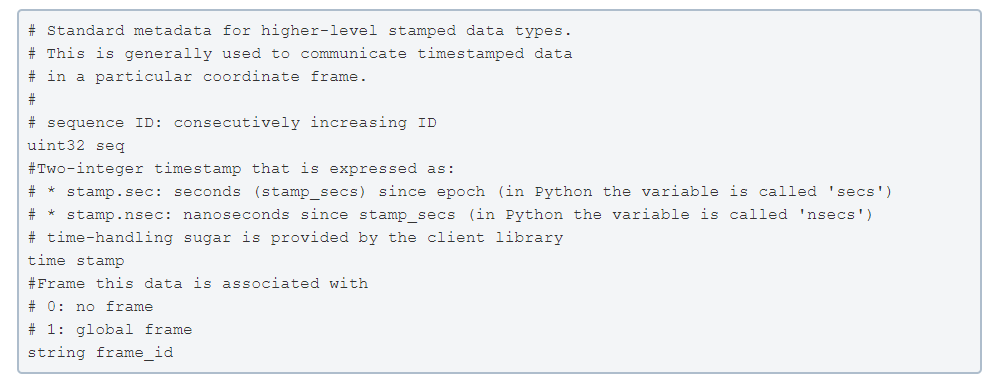
\includegraphics[width=\textwidth]{Images/msgheader.png}
        \caption{Message Header}
        \label{fig:my_label}
    \end{figure}
\end{itemize}
\subsubsection{bags}
Bags are a format for saving and playing back ROS message data. Bags are an important mechanism for storing data, such as sensor data, that can be difficult to collect but is necessary for developing and testing algorithms.
\subsubsection{package}
\href{http://wiki.ros.org/Packages}{Packages} might contain ROS nodes, ROS-independent library, a dataset, configuration files, a third-party software. Packages are created by hand or with tools like \textbf{catkin\_create\_pkg}. ROS package is a directory desended from \textit{ROS\_PACKAGE\_PATH} in \textit{\href{http://wiki.ros.org/ROS/EnvironmentVariables}{\underline{ROS Environment variable}}} that has a \href{http://wiki.ros.org/Manifest}{\textit{package.xml}} file in it.\\
ROS packages commonly contain the following strucutes.
\begin{itemize} 
    \item \textit{include/package\_name}: C++ incude header (make sure it export in CMakeLists.txt) 
    \item \textit{msg}/: folder contain Message(msg) types
    \item \textit{src/package\_name/}: source file, especially Python source that are exported to other packages
    
    %Do not know why if we use \textit here will cause error of `undefined control sequence` but change to \emph get rid of it
    \item \emph{scripts/}: executabe scripts
    \item \emph{CMakeList.txt}: CMake build file
    \item \emph{package.xml}: Package
    \underline{\href{http://wiki.ros.org/catkin/CMakeLists.txt}{catkin/CMakeLists.txt}}
\end{itemize}
There are few tools that help to manage the packages
\begin{itemize}
    \item \textit{rospack}: find and retrieve information about packet
    \item \textit{catkin\_create\_package}: create a new package
    \item \textit{catkin\_make}: build a workspace of package
    \item \textit{rosdep}: install system dependencies of a package
\end{itemize}
\subsubsection{catkin\_make}
A convenience tool for buidling code in workspace. Here we use\\
\textbf{\emph{\$ cd \~/catkin\_ws}}\\
\textbf{\emph{\$ catkin\_make}}\\
to compile and build our workspace. After running \emph{\textbf{catkin\_make}} we have 2 folder \emph{build} and \emph{devel} in our root of catkin workspace. The \emph{build} folder is where \emph{cmake} and \emph{make} are invoke, and the devel folder contains any generated files and targets, plus setup *.sh file so that you can use it like it is installed.

\subsubsection{package.xml}
A \textbf{package manifest} XML file that must be included with any catkin-compliant package's root folder that defines that package's properties such as package name, version number, author, maintainers and dependencies on other catkin package.\\
Some required tags include\\
\begin{itemize}
% Why <> cannot be compiled?
    \item \textit{name}: <name> of package
    \item \emph{<version>}: version of package
    \item \emph{<description>}: description of package content
    \item \emph{<maintainer>}: the name of person(s) that is/are maintaining the package
    \item \emph{<license>}: software license(s) (e.g GPL,BSD,ASL) under which code is release 
\end{itemize}

\subsection{Installing software}
First, operating system should be installed, for example (L)Ubuntu 16.04 minimal. Instructions can be found on Ubuntu website, for example: \url{https://help.ubuntu.com/community/Lubuntu/Documentation/MinimalInstall}. 
\\
Instructions for installing ROS can be found in \url{http://wiki.ros.org/kinetic/Installation/}.\\
Brief list of commands:
*adjust usernames etc. according to the local user, here openkin or pi*\\
\\
\# For raspbian jessie source installation: \# enough swap for build to succeed \\
\\
sudo fallocate -l 2G /var/swap2 \\ 
\\
sudo chmod 600 /var/swap2 \\
\\
sudo swapon /var/swap2 \\
\\
sudo sh -c 'echo "deb http://packages.ros.org/ros/ubuntu \$(lsb\_release -sc) main" > /etc/apt/sources.list.d/ros-latest.list' \\
\\
sudo apt-key adv --keyserver 'hkp://keyserver.ubuntu.com:80' --recv-keyC1CF6E31E6BADE8868B172B4F42ED6FBAB17C654 \\
\\
sudo apt-key del 421C365BD9FF1F717815A3895523BAEEB01FA116 \\
\\
sudo apt-get install python-rosdep python-rosinstall-generator python-wstool python-rosinstall build-essential git libgps-dev i2c-tools libi2c-dev \\
\\
sudo rosdep init \\
\\
rosdep uodate \\
\\
cd \\ 
\\
mkdir ros\_catkin\_ws \\
\\
cd ros\_catkin\_ws \\
\\
rosinstall\_generator ros\_comm --rosdistro kinetic --deps --wet-only --tar > kinetic-ros\_comm-wet.rosinstall \\
\\
roslocate info common\_msgs --distro=kinetic >> kinetic-ros\_comm-wet.rosinstall \\
\\
roslocate info tf --distro=kinetic >> kinetic-ros\_comm-wet.rosinstall \\
\\
roslocate info tf2 --distro=kinetic >> kinetic-ros\_comm-wet.rosinstall \\
\\
roslocate info diagnostic\_updater --distro=kinetic >> kinetic-ros\_comm-wet.rosinstall \\
\\
roslocate info actionlib --distro=kinetic >> kinetic-ros\_comm-wet.rosinstall \\
\\
roslocate info python\_orocos\_kdl --distro=kinetic >> kinetic-ros\_comm-wet.rosinstall \\
\\
roslocate info bondcpp --distro=kinetic >> kinetic-ros\_comm-wet.rosinstall \\
\\
nano kinetic-ros\_comm-wet.rosinstall \\
\\
\textbf{\emph{add to the end of file: - git: local-name:}} \\
\\
rosbag\_migration\_rule uri: \\
https://github.com/ros/rosbag\_migration\_rule.git\\
version: master \\
\*
\\
roslocate info pluginlib --distro=kinetic >> kinetic-ros\_comm-wet.rosinstall \\
\\
roslocate info angles --distro=kinetic >> kinetic-ros\_comm-wet.rosinstall \\
\\
roslocate info class\_loader --distro=kinetic >> kinetic-ros\_comm-wet.rosinstall \\
\\
wstool init -j4 src kinetic-ros\_comm-wet.rosinstall \\
\\
(sudo cp /usr/share/cmake-3.0/Modules/FindEigen3.cmake /usr/share/cmake-3.6/Modules/) \\
\\
rosdep install --from-paths src --ignore-src --rosdistro kinetic -y \\
\\
sudo mkdir -p /opt/ros/kinetic \\
\\
sudo chmod -R 777 /opt/ros \\
\\
sudo chown -R pi:pi /opt/ros \\
\\
./src/catkin/bin/catkin\_make\_isolated --install --install-space /opt/ros/kinetic -DCMAKE\_BUILD\_TYPE=Release \\
\\
cd\\
\\
\# Normal ubuntu, skip if from source\\
\\
The complete image of Ubuntu 16-04 with ROS kinetic already installed for raspberry pi 3 can be found at \url{https://ubiquity-pi-image.sfo2.cdn.digitaloceanspaces.com/2020-11-07-ubiquity-xenial-lxde-raspberry-pi.img.xz}\\
\\
sudo sh -c 'echo "deb http://packages.ros.org/ros/ubuntu \$(lsb\_release -sc) main" > /etc/apt/sources.list.d/ros-latest.list' 
\\
sudo apt-key adv --keyserver 'hkp://keyserver.ubuntu.com:80' --recv-keyC1CF6E31E6BADE8868B172B4F42ED6FBAB17C654 \\
\\
sudo apt-key del 421C365BD9FF1F717815A3895523BAEEB01FA116 \\
\\
sudo apt-get update\\
\\
rosdep update\\
\\
source ~/.bashrc\\
\\
sudo apt-get install libgps-dev libi2c-dev ntpdate\\
\\
sudo apt-get upgrade\\
\\
\\
\# Same for here\\
\\
% Not need to init catkin workspace anymore
catkin\_make\\
\\
source devel/setup.bash\\
\\
\textbf{\#If you start from here with fetching from the complete datalogger image}\\
\\
cd catkin\_ws/src\\
\\
ln -s /home/openkin/openkin/nodes/ascii\_logger/ascii\_logger\\
\\
ln -s /home/openkin/NewGaitMaven/nodes/vectornav vectornav \\
\\
\# for rpi \\
\\cd\\
\\
wget https://github.com/joan2937/pigpio/archive/master.zip\\
\\
unzip master.zip \\
\\
cd pigpio-master \\
\\
make -j4 \\
\\
sudo make install\\
\\
cd ~/catkin\_ws \\
\\
catkin\_make\\
\\
sudo visudo \\
\\
\textbf{*add line at the end: “openkin ALL=(ALL:ALL) NOPASSWD: ALL”*}\\
\\
sudo apt-get install screen ppp usb-modeswitch\\
\\
\textbf{\#if using E160E or similar }\\
\\
wget http://www.sakis3g.com/downloads/sakis3g.tar.gz\\
\\
tar -xzvf sakis3g.tar.gz\\
\\
sudo mv sakis3g /usr/bin/sakis3g \\
\\
sudo chown root:root /usr/bin/sakis3g\\
\\
sudo chmod +x /usr/bin/sakis3g \\
\\
\textbf{*if e3372 doesn’t work out of the box*}\\
\\
\textbf{*remove old usb\_modeswitch*}\\
\\
\textbf{*install tcl, libusb-1.0-0-dev etc.*}\\
\\
\textbf{*download latest usb\_modeswitch http://www.draisberghof.de/usb\_modeswitch/\#install*}\\
\\
\textbf{*sudo make install*}\\
\\
\\
\\
\textbf{Here we start to install git lfs for data storage}
% Add install golang and gitlfs
\\
\\
\\
cd \~/openkin/NewGaitMaven/linux-shutdown\\
\\
make\\
\\
\\
\\
% Enable automatic measurement
sudo nano /etc/rc.local\\
\\
\textbf{*add line before exit 0:}\\
\textit{“su -c “/home/openkin/NewGaitMaven/start\_script.sh” openkin}\\
\\
\textbf{*for rpi add shutdown\_flip*}\\
\\
\textbf{*check permissions for serial device, pi: /boot/cmdline.txt: remove serial terminal*}\\
\\
\textbf{*add source’s to .bashrc*}\\
\\
\textbf{*check usernames and folders in measurement.sh*}\\
\\
\\
\\
\# \textbf{For mtmanager}\\
\\
sudo apt-get install libqtopengl5 \\
\\
\textbf{*download mtmanager, extract, symlink to /usr/local/bin *}\\
\\
\subsection{3D Printed Cases}
Models can be found in 3D folder. They can be redesigned with SolidWork/FreeCad. FreeCad can be download for free. However, SolidWork require license from university and can be installed from IT-helpdesk.
\textbf{Some information and settings for printers} \\
Get start by running the script 
C:$\backslash$Minifactory$\backslash$Config$\backslash$first\_time\_config.bat.
Then press any key to continue\\
\\
Open Minifactory\\
\textbf{Step 1}: Start connect Z-calibration\\
\textbf{Step 2}: Run the nozzle up/down by pressing the arrow button until the paper slightly rubs between the nozzle and the print bed. Confirm height with “Ready” button. The height should be around 150cm\\
In manual control tab, uncheck the flowrate, bed temperature, extruder 1, extruder 2,. We mostly use extruder 1 for printing, the temperature is around 200 degree celsius.  

In object placement, add object and rotate it that its suitable (not need to much support )
In slicer tab, choose Slicer as Slic 3r or CuraEngine (prefered). If CuraEngine, the quality should be 0.2 mm and support everywhere.. The Filament setting is PLA for both extruder.

The preview tab can show each layer in real-time printing. Also, it shows the estimated print time, layer counts. Finally press Start Print.

\section{Usage}
\subsection{VectorNav}
The datalogger is off, if light is not on. The 4G modem should also be connected to the USB port before turning the logger on. The logger can be turn on by pressing the power button on the battery, inserting the battery to the case and connecting USB-cable to the battery. The logger will turn on and off the red and green leds when powering up respectively. When the logger acquire the internet connection, the green led is turned on. When the logger is synchronizing github/gitlab server, the green led is flashing\\
\\
When the logger has been on for a while and the green led is on, the logger is ready for starting measurement. The measurement can be started by disconnecting the 4G modem. 
The green led goes off and after a while, the red should start blinking if the VectorNav does not have fix, or if everything seem to be fine, the red led is turned on. It is still recommend to wait for GPS to acquire better stability, but the recording is running.\\
\\
When measurement are done, the recording can be stopped by reconnecting the 4G modem. The red led shuts off and the green led starts to blink as files are upload to github/gitlab. When the upload is done, the green led stabilize.\\
\\
The logger can be turn off by turning the power/shutdown switch off, and waiting for 10-30 seconds for all lights to go off. When logger is off, the USB power cable can be disconnected with care, and battery removed.\\
\\
Note: JYU version has reverse switch direction compared to other loggers, on is out, off is towards the antenna.

\section{SSH access}
The datalogger have SSH server running, and they can be accessed by connecting the datalogger via ethernet. The network should have DHCP to give IP address for the datalogger. For example internet sharing on Mac and Linux can be used for connecting the datalogger straight to the computer.\\
\\
The IP of the datalogger can possibly found using \textit{nmap}: \textit{nmap -sn 192.168.2.1-255} where IP range is subnet defined for network. The SSH connection can be mad with command \textit{ssh pi$@$192.168.2.3} where IP is the IP of the datalogger, and pi is the username.\\
\\
Username for Raspberry Pi based datalogger is pi. Password is raspberry for pi and openkin for openkin.\\
\\
\end{document}